\documentclass[tikz,border=2pt]{standalone}
\usepackage{amsmath,amssymb}
\usepackage{pgfplots}
\pgfplotsset{compat=1.18}
\usetikzlibrary{arrows.meta}

\begin{document}
% f(x) = x^3 - 3x + 1 on [a, b] = [-2.1, 2.1]: f(a) = -1.961, f(b) = 3.961. The level y = 2.1 lies
% between them and is reached at c1 = -1.5066, c2 = -0.3858, c3 = 1.8924.
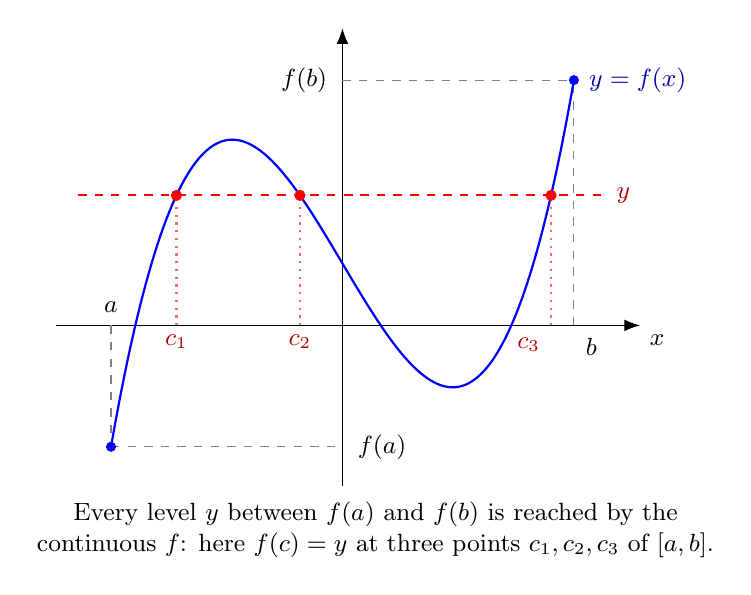
\begin{tikzpicture}[every node/.style={font=\small}]
	\begin{axis}[
		width=9cm, height=7.4cm,
		axis lines=middle, axis line style={-{Latex[length=2mm]}},
		xmin=-2.6, xmax=2.7, ymin=-2.6, ymax=4.8,
		xtick=\empty, ytick=\empty,
		xlabel={$x$}, xlabel style={below right},
		samples=200, clip=false
		]
		\addplot[gray, dashed] coordinates {(-2.1,0) (-2.1,-1.961)};
		\addplot[gray, dashed] coordinates {(2.1,0) (2.1,3.961)};
		\addplot[gray, dashed] coordinates {(-2.1,-1.961) (0,-1.961)};
		\addplot[gray, dashed] coordinates {(0,3.961) (2.1,3.961)};
		\addplot[red, dashed, thick, domain=-2.4:2.4] {2.1};
		\addplot[blue, thick, domain=-2.1:2.1] {x^3-3*x+1};
		\addplot[only marks, mark=*, mark size=1.6pt, blue] coordinates {(-2.1,-1.961) (2.1,3.961)};
		\addplot[only marks, mark=*, mark size=1.8pt, red] coordinates {(-1.5066,2.1) (-0.3858,2.1) (1.8924,2.1)};
		\addplot[red!60, dotted, thick] coordinates {(-1.5066,0) (-1.5066,2.1)};
		\addplot[red!60, dotted, thick] coordinates {(-0.3858,0) (-0.3858,2.1)};
		\addplot[red!60, dotted, thick] coordinates {(1.8924,0) (1.8924,2.1)};
		\node[anchor=south, font=\small] at (axis cs:-2.1,0.05) {$a$};
		\node[anchor=north west, font=\small] at (axis cs:2.12,-0.05) {$b$};
		\node[anchor=north, red!70!black, font=\small] at (axis cs:-1.5066,0) {$c_1$};
		\node[anchor=north, red!70!black, font=\small] at (axis cs:-0.3858,0) {$c_2$};
		\node[anchor=north east, red!70!black, font=\small] at (axis cs:1.88,-0.05) {$c_3$};
		\node[anchor=west, font=\small] at (axis cs:0.05,-1.961) {$f(a)$};
		\node[anchor=east, font=\small] at (axis cs:-0.05,3.961) {$f(b)$};
		\node[anchor=west, red!70!black] at (axis cs:2.4,2.1) {$y$};
		\node[blue!70!black, anchor=west] at (axis cs:2.15,3.96) {$y=f(x)$};
	\end{axis}
	\node[anchor=north, align=flush center, text width=8.6cm] at ([yshift=-2pt]current bounding box.south) {Every level $y$ between $f(a)$ and $f(b)$ is reached by the continuous $f$: here $f(c)=y$ at three points $c_1,c_2,c_3$ of $[a,b]$.};
\end{tikzpicture}
\end{document}
